\subsection{Librer\'ia b\'asica para sistemas de implicaciones}
Se va a intentar que este paquete de funciones pueda perdurar en el tiempo, y para ello, 
se a realizado una librer\'ia b\'asica para intentar modularizar el c\'odigo y que sea lo 
m\'as legible posible a la hora de poder comprenderlo.

En esta librer\'ia b\'asica se encuentran diferentes funciones que se usar\'an bastante a lo largo de este TFG, a continuaci\'on 
se van a detallar una a una.




%%% initialize.setOfAttributes %%%
\subsubsection{Inicializar conjunto de atributos}

    \textbf{Descripci\'on}

    Esta funci\'on se utilizar\'a para inicializar un conjunto de datos, es decir, se le va a pasar un subconjunto 
    de todos los atributos que componen a un grupo de implicaciones, adem\'as del conjunto completo de los atributos. 
    
    Dentro de esta se va a utilizar la funci\'on encode para convertir el subconjunto de atributos en un objeto itemMatrix, y de esta 
    forma poder trabajar con ellos en los diferentes algoritmos que se van a desarrollar a lo largo de este TFG.

    Es decir, con esta funci\'on lo que se consigue es tener un conjunto de atributos con la estructura adecuada para poder trabajar con \'el.
    \\

    
    \textbf{C\'odigo}
    
    \lstinputlisting{r_code/basicLibrary/initialize.setOfAttributes.R}
    
    
    \textbf{Ejemplo}

    Para que se entienda mejor esta funci\'on, se va a plantear un ejemplo:

    \begin{figure}[H]
        \centering
        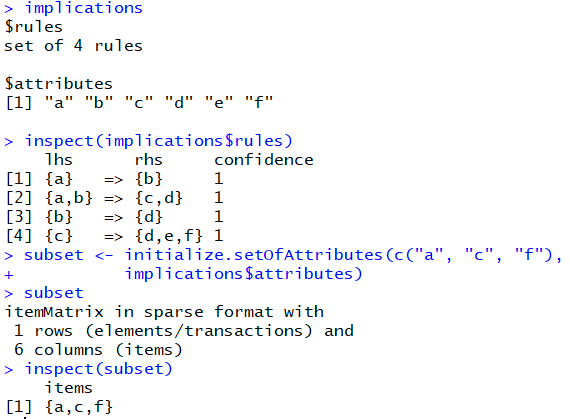
\includegraphics{InicializarConj}
        \caption{Ejemplo de inicializar conjunto de atributos}
        \label{fig:InicializarConj}
    \end{figure}

    En la variable implications se tiene un conjunto de 4 reglas y el conjunto de atributos que las componen.
    Al usar la funci\'on descrita en este punto, pas\'andole un subconjunto de todos los atributos, en este caso \{a,c,f\}, y 
    el conjunto total de los atributos, nos devuelve un itemMatrix. 
    
    Dicho itemMatrix est\'a compuesto s\'olo por esos tres atributos, aunque va a contener la informaci\'on de todos los que 
    componen las reglas; ya que deben estar para poder usar algunas funciones como uni\'on o intersecci\'on.



%%% is.singleton %%%
\subsubsection{Conjunto unitario}

    \textbf{Descripci\'on}
    
    Un conjunto unitario es aquel que tiene un s\'olo elemento. Por lo que esta funci\'on 
    devolver\'a TRUE si la longitud del conjunto que se le pase es igual a 1, o FALSE en caso 
    contrario.

    Esta es una funci\'on a la que se le puede pasar por par\'ametro una lista, un vector, 
    un conjunto de reglas o cualquier otro conjunto de elementos al que se le pueda aplicar la funci\'on 
    length().
    \\


    \textbf{C\'odigo}

    \lstinputlisting{r_code/basicLibrary/is.singleton.R}

    
    \textbf{Ejemplo}

    En este caso, se van a proponer tres ejemplos diferentes para poder entender el comportamiento de esta funci\'on:

    \begin{figure}[H]
        \centering
        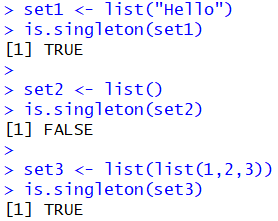
\includegraphics{singleton}
        \caption{Ejemplos de conjuntos unitarios}
        \label{fig:singleton}
    \end{figure}

    En el primero ejemplo, se puede observar que el conjunto es unitario porque est\'a compuesto por una sola cadena de caracteres. 
    Es decir, no cuenta caracter a caracter, sino la cadena, luego est\'a formado por un solo elemento y el resultado es TRUE.

    En el segundo ejemplo, tenemos una lista vac\'ia, por lo que como no tiene ning\'un elemento, el resultado es FALSE porque no es unitario.

    Por \'ultimo, se tiene una lista que contiene a otra lista con tres elementos dentro de ella. En este caso, se podr\'ia pensar que 
    no es unitario al ver los tres elementos, pero no, ya que el elemento que estamos estudiando es el primero, y este contiene solo una lista 
    en \'el, por lo que el resultado es TRUE, ya que s\'i es unitario.



%%% union.sets %%% 
\subsubsection{Uni\'on}

    \textbf{Descripci\'on}

    La uni\'on de dos conjuntos es una operaci\'on que devolver\'a otro conjunto formado por 
    todos los elementos de los dos conjuntos iniciales. Si un elemento se encuentra en los dos 
    conjuntos, s\'olo aparecer\'a una vez en el resultante.

    \[
    A \cup B = \{x\in U ~ | ~ x\in A ~ \'o ~ x\in B \}
    \]
    

    Esta funci\'on se usar\'a para la uni\'on de elementos de la clase itemMatrix, ya que lo que 
    se usa es itemUnion, una funci\'on perteneciente al paquete arules.
    \\


    \textbf{C\'odigo}

    \lstinputlisting{r_code/basicLibrary/union.sets.R}
    
    \textbf{Ejemplo}

    \begin{figure}[H]
        \centering
        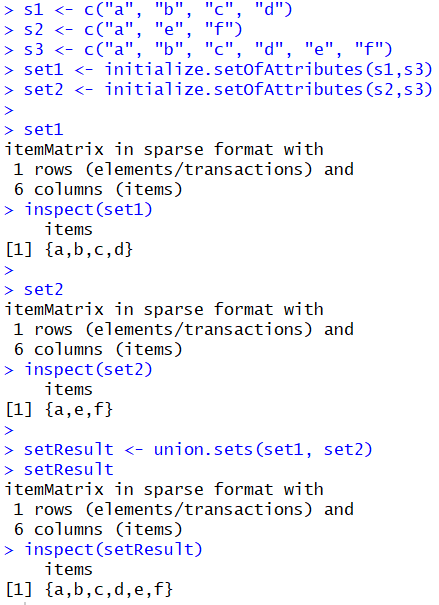
\includegraphics{union}
        \caption{Ejemplo de uni\'on de conjuntos}
        \label{fig:union}
    \end{figure}

    A continuaci\'on se va a explicar el anterior ejemplo paso a paso, ya que en \'el se han realizado varios pasos.

    Primero, se ha comenzado declarando tres vectores diferentes. Los dos primeros van a ser los dos conjuntos a unir, y el 
    tercero es la uni\'on de todas las variables. Despu\'es, se utiliza la funci\'on explicada anteriormente para convertir ambos 
    vectores en itemMatrix.

    Segundo, se observa que ambos conjuntos son de la estructura itemMatrix, con el mismo n\'umero de columnas. Esto es algo muy 
    importante, y por eso se ha usado la funci\'on initialize.setOfAttributes, ya que para utilizar la uni\'on, los elementos deben 
    estar en los dos conjuntos como informaci\'on, tal y como se vi\'o en la estructura de datos itemMatrix.

    Por \'ultimo, se realiza la uni\'on e inspeccionamos la variable resultante, y se comprueba que se ha realizado correctamente.




%%% intersection.sets %%% 
\subsubsection{Intersecci\'on}

    \textbf{Descripci\'on}
    
    La intersecci\'on de dos conjuntos A y B devolver\'a otro conjunto resultante U con los elementos 
    que se encuentren en ambos conjuntos iniciales. Es decir, el conjunto U estar\'a formado por los elementos 
    que est\'en tanto en A como en B.

    \[
    A \cap B = \{x\in U ~ | ~ x\in A ~ y ~ x\in B \}
    \]

    En este caso, tambi\'en se usar\'a con la estructura de datos itemMatrix que es la usada mayoritariamente con implicaciones 
    como ya se ha especificado antes.
    \\


    \textbf{C\'odigo}

    \lstinputlisting{r_code/basicLibrary/intersection.sets.R}
    
    \textbf{Ejemplo}

    Para el ejemplo de esta funci\'on se van a utilizar los mismos conjuntos del ejemplo de la anterior funci\'on:

    \begin{figure}[H]
        \centering
        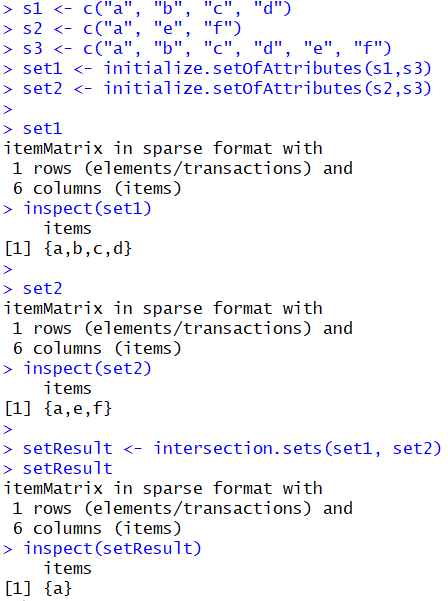
\includegraphics{interseccion}
        \caption{Ejemplo de intersecci\'on de conjuntos}
        \label{fig:interseccion}
    \end{figure}

    Para comenzar el ejemplo, se han realizado los mismos pasos que en el anterior, se declaran las variables y se convierten a 
    itemMatrix. 
    Por \'ultimo, se realiza la intersecci\'on de ambos conjuntos y vemos como el resultado es \'unicamente del elemento que se encuentra 
    en ambos conjuntos.




%%% difference.sets %%% 
\subsubsection{Diferencia}

    \textbf{Descripci\'on}

    La diferencia de dos conjuntos da como resultado otro conjunto con los elementos que resultan de 
    eliminar a los elementos que forman el primer conjunto, los del segundo. Es decir, se obtendr\'ian 
    todos elementos del primer conjunto que no est\'an en el segundo.

    \[
    A - B = \{x\in A ~ y ~ x\notin B \}
    \]

    De nuevo, en nuestra funci\'on se usa una del paquete arules para poder utilizar la gran mayor\'ia de estructuras 
    que sean compatibles con restar elementos.
    \\


    \textbf{C\'odigo}

    \lstinputlisting{r_code/basicLibrary/difference.sets.R}
    
    \textbf{Ejemplo}

    Para ilustrar bien esta funci\'on, vamos a volver a utilizar los conjuntos usados en la uni\'on e intersecci\'on para comprobar 
    cu\'al ser\'ia el resultado al realizar la diferencia de estos conjuntos.

    \begin{figure}[H]
        \centering
        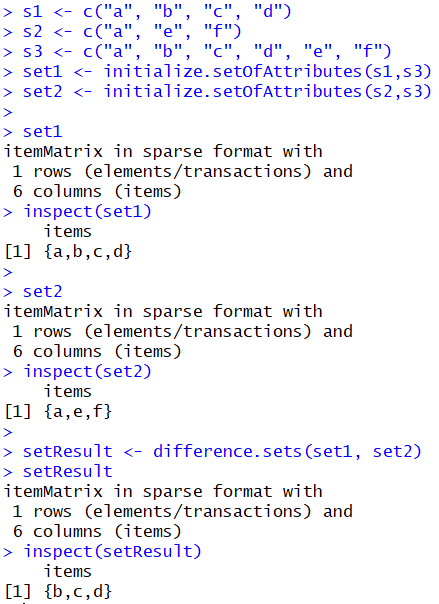
\includegraphics{diferencia}
        \caption{Ejemplo de diferencia de conjuntos}
        \label{fig:diferencia}
    \end{figure}

    En este caso, se vuelve a realizar todo de la mismo forma que en los anteriores casos, pero usamos la funci\'on difference.sets, y 
    con ella obtenemos como resultado un nuevo conjunto, en el que se encuentran los elementos del primer conjunto, eliminando los que 
    tambi\'en est\'en en el segundo.



%%% is.included %%% 
\subsubsection{Inclusi\'on}

    \textbf{Descripci\'on}

    Un conjunto A est\'a incluido en un conjunto B, si A es subconjunto de B. Por lo que esta funci\'on 
    devolver\'a TRUE si cumple dicha propiedad, o FALSE en caso contrario.

    \[
    A \subseteq B ~ | ~  \forall ~ x \in A \to x \in B 
    \]

    De nuevo, esta funci\'on se utilizar\'a con elementos de la clase itemMatrix.
    \\


    \textbf{C\'odigo}

    \lstinputlisting{r_code/basicLibrary/is.included.R}


    \textbf{Ejemplo}

    \begin{figure}[H]
        \centering
        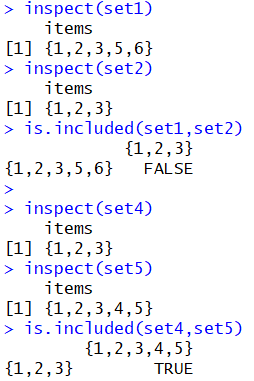
\includegraphics{inclusion}
        \caption{Ejemplos de inclusi\'on de conjuntos}
        \label{fig:inclusion}
    \end{figure}

    En este caso, se van a proponer dos ejemplos:

    En el primero no se cumple que el set1 est\'e incluido en el set2, aunque s\'i se cumplir\'ia al contrario, pero la inclusi\'on no es 
    una funci\'on que cumpla la propiedad sim\'etrica, luego en este caso el resultado es FALSE.

    En el segundo ejemplo s\'i que se cumple que el primer conjunto est\'e incluido en el segundo. Como se puede observar da igual el orden 
    en el que es\'en los elementos.



%%% is.empty.set %%% 
\subsubsection{Vac\'io}

    \textbf{Descripci\'on}

    Un conjunto es vac\'io si no contiene ning\'un elemento. Es decir, si su el tama\~no del conjunto es 0, 
    podemos decir que est\'a vac\'io. 
    \[
    A = \{ \} = \emptyset
    \]

    \textbf{C\'odigo}

    \lstinputlisting{r_code/basicLibrary/is.empty.set.R}

    \textbf{Ejemplo}

    \begin{figure}[H]
        \centering
        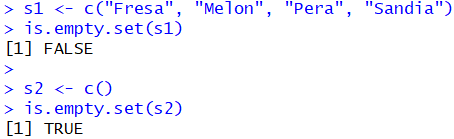
\includegraphics{vacio}
        \caption{Ejemplos de conjuntos vac\'ios}
        \label{fig:vacio}
    \end{figure}

    En el primer ejemplo, se puede ver que la funci\'on devuelve FALSE porque el conjunto contiene elementos.

    En cambio, en el segundo, el vector no contiene elementos, por lo que la funci\'on devuelve TRUE porque el conjunto no tiene 
    elementos.


    %%% equals.sets %%% 
\subsubsection{Igualdad}

    \textbf{Descripci\'on}

    Dos conjuntos A y B son iguales si su longitud es la misma, y si para cada elemento de A, existe uno igual 
    en B y para cada elemento de B existe uno igual en A.

    Ya que, seg\'un el axima de extensionalidad:

    \[
    \forall A, B : \forall x, (x \in A \Leftrightarrow x \in B) \to A = B
    \]


    \textbf{C\'odigo}

    \lstinputlisting{r_code/basicLibrary/equals.sets.R}


    \textbf{Ejemplo}

    \begin{figure}[H]
        \centering
        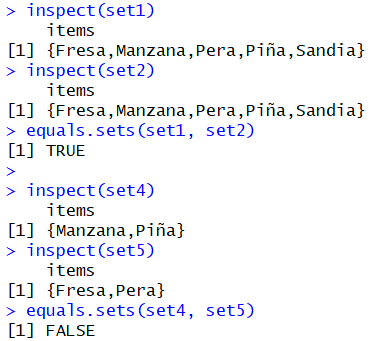
\includegraphics{igualdad}
        \caption{Ejemplos de igualdad de conjuntos}
        \label{fig:igualdad}
    \end{figure}

    De nuevo, se plantean dos ejemplos. En el primero, el resultado es TRUE, ya que visualmente se puede comprobar que ambos conjuntos son 
    iguales.

    En el segundo caso, la funci\'n devuelve FALSE porque los conjuntos no son iguales.


%%%%%%%%%%%%%%%%%%%%%%%%%%%%%%%%%%%%%%%%%%%%%%%%%%%%%%%%%%%%%%%%%%%%%%%%%%%%%%%%%%%%%%%%%%%%%%%%%%%%%%%%%%%%%%%%%%%%%%%%


%%% remove.imp %%% 
\subsubsection{Eliminar implicaci\'on}

    \textbf{Descripci\'on}

    Una de las tareas m\'as importantes de este TFG es trabajar con implicaciones. Una de las operaciones m\'as habituales 
    va a ser la de eliminar una implicaci\'on de un conjunto. Para ello, se ha definido la siguiente funci\'on, pas\'andole 
    como par\'ametros el conjunto de implicaciones y la posici\'on de la que se desea eliminar, devolver\'a un conjunto sin 
    dicha implicaci\'on.
    \\


    \textbf{C\'odigo}

    \lstinputlisting{r_code/basicLibrary/remove.imp.R}


    \textbf{Ejemplo}

    \begin{figure}[H]
        \centering
        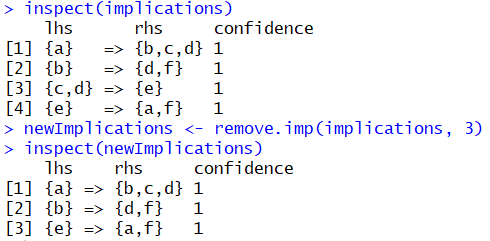
\includegraphics{removeImp}
        \caption{Ejemplo de eliminar implicaci\'on}
        \label{fig:removeImp}
    \end{figure}

    En este ejemplo, tenemos un conjunto inicial implications con cuatro implicaciones diferentes. A continuaci\'on se usa la 
    funci\'on remove.imp y con ella eliminamos la tercera.

    Finalizamos comprobando que efectivamente, en el nuevo conjunto solo se tienen tres implicaciones, quitando la tercera del conjunto 
    inicial.



%%% remove.all %%% 
\subsubsection{Vaciar conjunto}

    \textbf{Descripci\'on}

    Otra funci\'on que puede ser \'util es vaciar un conjunto. Se podr\'ia pensar que igualando el conjunto a nulo, 
    se podr\'ia obtener el resultado que se quiere conseguir. Pero no es as\'i, ya que lo que se quiere es un conjunto sin 
    elementos, pero que siga manteniendo su estructura de conjunto, no algo nulo. 
    
    Para ello, en esta funci\'on, vamos a devolver la posici\'on 0 del conjunto que se quiere vaciar. Recordemos, que en el 
    lenguaje R los arrays, listas y dem\'as estructuras de conjuntos comienzan en 1 y no en 0 como la gran mayor\'ia de lenguajes.
    Por lo que al devolver esta posici\'on, el resultado que se obtiene es el conjunto que se le hab\'ia pasado, pero sin ning\'un 
    elemento.
    \\


    \textbf{C\'odigo}

    \lstinputlisting{r_code/basicLibrary/remove.all.R}

    \textbf{Ejemplo}

    \begin{figure}[H]
        \centering
        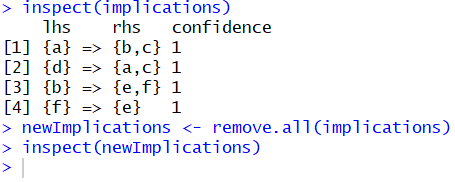
\includegraphics{removeAll}
        \caption{Ejemplo de vaciar conjunto}
        \label{fig:removeAll}
    \end{figure}

    En este caso, tenemos un conjunto de implicaciones, y si vaciamos dicho conjunto, el resultado el vac\'io ya que el nuevo 
    conjunto resultante no contiene ninguna implcaci\'on.




%%% add.imp.k %%% 
\subsubsection{A\~nadir implicaci\'on en posici\'on}

    \textbf{Descripci\'on}

    Igual que se puede querer eliminar una implicaci\'on, tambi\'en ser\'a posible a\~nadir una nueva en una determinada posici\'on 
    del conjunto. Para esta funci\'on necesitamos como par\'ametros, el conjunto que se quiere ampliar, la parte izquierda de la nueva 
    implicaci\'on, la derecha y la posici\'on que queremos que ocupe en el conjunto.

    Luego, en dicha funci\'on, lo primero que se hace es crear una nueva regla, con las dos partes que le hemos pasado. A continuaci\'on, 
    unimos en un mismo conjunto, todas las implicaciones que se ten\'ian en las posiciones anteriores a la nueva que se quiere insertar, 
    la nueva implicaci\'on, y las restantes que se encontraban en posiciones posteriores. Y finalmente, se devuelve este conjunto.
    \\


    \textbf{C\'odigo}

    \lstinputlisting{r_code/basicLibrary/add.imp.k.R}

    \textbf{Ejemplo}



%%% add.imp %%% 
\subsubsection{A\~nadir implicaci\'on}

    \textbf{Descripci\'on}

    Al igual que en el caso anterior se quer\'ia a\~nadir una implicaci\'on en una determinada posici\'on, puede que d\'e igual 
    el lugar en el que se inserte. Por lo que esta funci\'on, inserta la nueva implicaci\'on en la \'ultima posici\'on del 
    conjunto. Como par\'ametros necesita los mismos que en el punto anterior, excepto la posici\'on a insertar.

    As\'i que, se crea la nueva implicaci\'on, con las dos partes que se le pasan como par\'ametros, y se le concatena al conjunto 
    inicial para devolver un conjunto ampliado con una nueva implicaci\'on.
    \\


    \textbf{C\'odigo}

    \lstinputlisting{r_code/basicLibrary/add.imp.R}


    \textbf{Ejemplo}



%%% new.imp %%% 
\subsubsection{Nueva implicaci\'on}

    \textbf{Descripci\'on}

    Con esta funci\'on, vamos a insertar una nueva implicaci\'on, al igual que en los dos puntos anteriores, pero esta vez 
    de una forma un poco m\'as compleja. Ya que, en este caso, se van a realizar varias comprobaciones.

    Para cada implicaci\'on perteneciente al conjunto, se va a comprobar si el antecedente es igual al que se quiere insertar.
    En caso negativo, se continuar\'a con la siguiente implicaci\'on; y en caso afirmativo, se comprobar\'a si los consecuentes son 
    iguales. En caso de que se cumplan ambas afirmaciones, quiere decir que la implicaci\'on que intentamos insertar en el conjunto, 
    ya se encuentra en \'el, por lo que se devolver\'a el conjunto inicial sin ning\'un cambio.

    En el caso de que los antecedentes sean iguales, y los consecuentes no, se sustituir\'a esa regla por una nueva, en la que el antecedente 
    queda igual, y el consecuente estar\'a formado por la uni\'on del que ya estaba en el conjunto, y el nuevo que se quiere insertar. Y con 
    esto, se devolver\'ia el nuevo conjunto.

    El \'ultimo caso que se podr\'ia dar, es aquel en el que ninguna implicaci\'on del conjunto tenga el mismo antecedente que el que se 
    quiere insertar, por lo que al finalizar la iteraci\'on por todo el conjunto, se insertar\'ia la nueva regla y devolver\'ia el conjunto 
    resultante.
    \\


    \textbf{C\'odigo}

    \lstinputlisting{r_code/basicLibrary/new.imp.R}


    \textbf{Ejemplo}


%%% read.left %%% 
\subsubsection{Leer antecedente}

    \textbf{Descripci\'on}

    Otra de las funciones b\'asicas a la hora de trabajar con implicaciones es poder obtener el antecedente de una determinada 
    implicaci\'on. Para ello, pas\'andole a esta funci\'on el conjunto que contiene a la implicaci\'on que queremos obtener, y su 
    posici\'on, nos devolver\'a el antecedente deseado.
    \\


    \textbf{C\'odigo}

    \lstinputlisting{r_code/basicLibrary/read.left.R}


    \textbf{Ejemplo}


%%% read.right %%% 
\subsubsection{Leer consecuente}

    \textbf{Descripci\'on}
    
    De igual forma que en el anterior punto, se puede querer obtener el consecuente de una implicaci\'on, luego, con el conjunto de 
    implicaciones y su posici\'on, esta funci\'on devolver\'a el consecuente de dicha implicaci\'on.
    \\


    \textbf{C\'odigo}

    \lstinputlisting{r_code/basicLibrary/read.right.R}

    \textbf{Ejemplo}


%%% substitute.imp %%% 
\subsubsection{Sustituir implicaci\'on}

    \textbf{Descripci\'on}

    La sustituci\'on de una implicaci\'on es una operaci\'on bastante \'util, ya que cuando se quieren unir dos implicaciones, puede que 
    se quiera que la nueva permanezca en un lugar determinado, para ello, esta funci\'on inserta la nueva implicaci\'on en el lugar que 
    se le indique. Como par\'ametros, necesita el conjunto de implicaciones, la posici\'on a cambiar, y los nuevos antedecente y consecuente.
    \\


    \textbf{C\'odigo}

    \lstinputlisting{r_code/basicLibrary/substitute.imp.R}

    %% Hay que revisar muy muy bien, como lo hace, creo que no sustituye, sino que añade y listo. 
    \textbf{Ejemplo}


%%% included.left %%% 
\subsubsection{Incluido en antecedente}

    \textbf{Descripci\'on}

    Si tenemos dos implicaciones A y B y se quiere comprobar si el antecedente de A est\'a incluido en el de B, se debe usar 
    esta funci\'on. Le pasamos como par\'ametros un conjunto de implicaciones, y dos posiciones de dicho conjunto. Se usar\'an 
    las funciones is.included y read.left para comprobar si un antecedente est\'a incluido en otro, devolver\'a TRUE en caso 
    afirmativo, y FALSE en el contrario.
    \\


    \textbf{C\'odigo}

    \lstinputlisting{r_code/basicLibrary/included.left.R}

    \textbf{Ejemplo}



%%% included.left.right %%% 
\subsubsection{Antecedente incluido en consecuente}

    \textbf{Descripci\'on}

    En una implicaci\'on, si el antecedente est\'a incluido en el consecuente se puede simplificar el consecuente, ya que 
    esto es algo trivial. Esta funci\'on, devolver\'a TRUE en el caso de que el antecedente est\'e incluido en el consecuente o 
    FALSE en el caso contrario. Para ello...

    ACLARAR QU\'E ES EXACTAMENTE LO QUE HACE, NO LO ENTIENDO
    \\


    \textbf{C\'odigo}

    \lstinputlisting{r_code/basicLibrary/included.left.right.R}


    \textbf{Ejemplo}


%%% delete.set.of.IS %%% 
\subsubsection{Eliminar implicaciones con consecuente vac\'io}

    \textbf{Descripci\'on}

    Si se tiene un conjunto de implicaciones y alguna de ellas tiene su consecuente vac\'io, esta implicaci\'on no va a 
    aportar ning\'un tipo de conocimiento a este conjunto, por lo que se deben eliminar. Para ello, se usar\'ia esta funci\'on, 
    la cual, pas\'andole como par\'ametro dicho conjunto, nos devolver\'a uno nuevo eliminando las implicaciones con su consecuente 
    vac\'io.
    \\


    \textbf{C\'odigo}

    \lstinputlisting{r_code/basicLibrary/delete.set.of.IS.R}


    \textbf{Ejemplo}


%%% size.set %%% 
\subsubsection{Tama\~no del conjunto}

    \textbf{Descripci\'on}

    Por tama\~no del conjunto, se entiende el n\'umero de elementos, repetidos o no, que lo componen. 
    Es decir, para calcular el tama\~no de un conjunto, se va a realizar la suma de los tama\~nos de cada una de 
    las implicaciones que forman el conjunto.
    \\


    \textbf{C\'odigo}

    \lstinputlisting{r_code/basicLibrary/size.set.R}

    \textbf{Ejemplo}



%%% cadinality.set %%% 
\subsubsection{Cardinalidad del conjunto}

    \textbf{Descripci\'on}

    La cardinalidad de un conjunto, se entiende como el n\'umero de implicaciones que lo componen. Es decir, lo que 
    tambi\'en se suele denominar como longitud del conjunto.
    \\


    \textbf{C\'odigo}

    \lstinputlisting{r_code/basicLibrary/cardinality.set.R}

    \textbf{Ejemplo}




%%% core %%% 
\subsubsection{Core}

    \textbf{Descripci\'on}

    A esta funci\'on se le pasa un conjunto de atributos Omega, junto con un conjunto de implicaciones Gamma. 
    Devolver\'a un conjunto de datos resultante de eliminar de Omega todos los atributos que se encuentren en los 
    consecuentes de las implicaciones que forman Gamma. 
    
    Esta no es precisamente una funci\'on b\'asica, pero se ha incluido en este apartado, ya que se utilizar\'a 
    en el algoritmo de claves minimales realizado en el segundo tomo de este TFG.
    \\


    \textbf{C\'odigo}

    \lstinputlisting{r_code/basicLibrary/core.R}

    \textbf{Ejemplo}




%%% body %%% 
\subsubsection{Body}

    \textbf{Descripci\'on}

    Al igual que en el punto anterior, esta funci\'on se utilizar\'a en el algoritmo para calcular claves minimales, aunque junto con 
    el anterior, se han incluido aqu\'i.

    Siendo Omega un conjunto de atributos, y Gamma un conjunto de implicaciones, se define la funci\'on body como la diferencia 
    de la uni\'on de los antecedentes de Gamma, menos el cierre del core de Omega y Gamma. 
    \\


    \textbf{C\'odigo}

    \lstinputlisting{r_code/basicLibrary/body.R}

    \textbf{Ejemplo}


